% !TEX root = ../main.tex

\chapter{基于halo2的SAT问题的约束系统}

本章提出基于halo2约束系统的零知识验证框架，分别针对SAT问题的不可满足性（UNSAT）和可满足性（SAT）两种情况设计算术化方案。对于UNSAT证明，我们提出挑战值编码技术，将变长子句压缩为单个有限域元素，实现高效的归结证明验证；对于SAT证明，我们设计双矩阵赋值存储方案，通过互斥性约束确保变量赋值的唯一性。这些技术创新使得验证复杂度与子句宽度和公式长度解耦，在保持零知识性的同时显著提升了验证效率。

\section{halo2算术电路系统}

halo2是由Zcash团队开发的零知识证明库，是PLONKish算术化方案的高效工程实现\cite{halo2}。halo2采用表格结构表示计算，将执行过程编码为有限域$\mathbb{F}$上的矩阵$M \in \mathbb{F}^{k \times n}$，矩阵中的每个元素均为有限域元素。有限域$\mathbb{F}$通常选取大素数阶的域（如$|\mathbb{F}| \approx 2^{256}$），以确保密码学安全性。

halo2的列类型分为三类，如表\ref{tab:halo2-columns}所示。Advice列存储私有见证，仅证明者可见，保证零知识性；Instance列存储公开输入输出，证明者和验证者均可见；Fixed列存储电路常量和选择器，在电路编译时确定。这种列类型的划分使得halo2能够在保持零知识性的同时，支持公开输入与私有见证的分离处理。

\begin{table}[htbp]
\centering
\bicaption{halo2列类型及其特性}{Column types and their properties in halo2}
\label{tab:halo2-columns}
\begin{tabular}{llll}
\toprule
\textbf{列类型} & \textbf{英文名称} & \textbf{可见性} & \textbf{用途} \\
\midrule
建议列 & Advice & 仅证明者可见 & 存储私有见证和中间计算值 \\
实例列 & Instance & 证明者和验证者均可见 & 存储公开输入和输出 \\
固定列 & Fixed & 证明者和验证者均可见 & 存储电路常量和选择器 \\
\bottomrule
\end{tabular}
\end{table}

在约束系统方面，halo2支持四种核心约束类型：门约束（Gate Constraints）通过自定义门实现灵活的算术运算编码；复制约束（Copy Constraints）通过置换论证确保不同位置的值相等；查找约束（Lookup Constraints）将元素成员关系验证归约为高效的多项式检查；置乱约束（Shuffle Constraints）验证两列元素作为多重集合的相等性。这四种约束的组合为构建复杂验证逻辑提供了强大的表达能力。

\section{基于halo2的归结证明系统}\label{sec:plonkish-zk-system}

本节提出基于halo2约束系统的零知识验证框架，实现UNSAT归结证明的隐私保护验证。我们设计挑战值编码技术，将变长子句压缩为单个有限域元素，使得验证复杂度与子句宽度解耦，在保持零知识性的同时显著提升验证效率。

\subsection{基于halo2的归结证明的编码方案}\label{sec:unsat-challenge-encoding}

归结证明验证的核心挑战在于如何在halo2框架内高效表示变长子句及其推导关系。传统的直接编码方法会导致约束数量随子句宽度线性增长，验证复杂度难以控制。我们提出基于挑战值的压缩编码方案，将每个子句——无论包含多少文字——编码为有限域中的单个元素。

\textbf{归结证明的形式化定义:}
设布尔公式$F$为合取范式（CNF），由$n$个子句组成，即$F = \{f_1, f_2, \ldots, f_n\}$，其中每个子句$f_i$是文字的析取。归结证明由三个部分组成：
\begin{itemize}
    \item \textbf{原始公式}$F^*$：待证明不可满足的CNF公式，包含$n$个子句。
    \item \textbf{导出子句序列}$D^* = \{d_1, d_2, \ldots, d_k\}$：通过归结规则从$F^*$逐步导出的子句序列，最终元素$d_k$为空子句$\bot$。
    \item \textbf{归结轨迹}$T^* = \{t_1, t_2, \ldots, t_{2k}\}$：记录每个导出子句的两个父子句，即$d_i$由$t_{2i-1}$和$t_{2i}$归结得到。
\end{itemize}

\textbf{文字到有限域的映射:}
在halo2框架中，所有数据必须表示为有限域$\mathbb{F}$中的元素。我们定义文字的编码规则如下：设布尔变量集合为$X = \{x_1, x_2, \ldots, x_m\}$，文字$\ell$编码为有限域元素$\ell \in \mathbb{F}$：
\begin{itemize}
    \item 正文字$x_j$编码为正整数：$\ell = j > 0$
    \item 负文字$\neg x_j$编码为负整数：$\ell = -j < 0$（在有限域中表示为$p - j$，其中$p$为域的阶）
\end{itemize}
这种编码保证了互补文字的和为零：$\ell(x_j) + \ell(\neg x_j) = j + (-j) = 0$，这一性质将在约束设计中被利用。子句$c$表示为编码文字的有序集合$c = \{\ell_1, \ell_2, \ldots, \ell_k\}$，每个子句附加唯一索引$i^* \in \mathbb{F}$以区分不同子句。

\textbf{挑战值编码方案:}
设$W = \max_{t \in T} |t|$为最大子句宽度。验证者在每次验证时生成随机挑战值向量$\tilde{\chi} = \{\chi_0, \chi_1, \ldots, \chi_W\} \subseteq \mathbb{F}$。子句$(i^*, c)$通过挑战值编码为单个域元素：
$$\text{Encode}(c, \tilde{\chi}) = i^* \cdot \chi_0 + \sum_{j=1}^{|c|} \chi_j \cdot \ell_j$$
其中$i^*$为子句索引，$\ell_j$为子句中第$j$个文字。对于长度小于$W$的子句，缺失位置的文字视为零。

\textbf{编码方案的安全性分析:}
该编码本质上是随机多项式求值。考虑两个不同的子句$c_1 \neq c_2$，其编码相等的概率为：
$$\Pr[\text{Encode}(c_1, \tilde{\chi}) = \text{Encode}(c_2, \tilde{\chi})] = \Pr\left[\sum_{j=0}^{W} \chi_j \cdot (\ell_{1,j} - \ell_{2,j}) = 0\right]$$
由于$c_1 \neq c_2$，根据Schwartz-Zippel引理，该概率至多为$W/|\mathbb{F}|$。在大有限域中（如$|\mathbb{F}| \approx 2^{256}$），该概率可忽略不计。

\textbf{编码效率优势:}
挑战值编码将子句间的包含关系验证从$O(W)$复杂度的逐元素比较降至$O(1)$的标量相等性检查。对于包含$|T|$个子句的归结轨迹，传统方法需要$O(|T| \cdot W)$次比较操作，而挑战值编码仅需$O(|T|)$次查找操作。

\subsection{基于halo2的归结证明的算术矩阵构造算法}\label{sec:unsat-matrix-construction}

基于挑战值编码方案，我们将归结证明映射到halo2矩阵结构。矩阵构造的目标是将原始公式$F$、导出子句$D$和归结轨迹$T$以及它们之间的推导关系，转化为有限域上的列向量和约束关系。halo2矩阵$M \in \mathbb{F}^{n \times m}$是一个有限域元素构成的二维表格，其中$n$为行数对应电路的执行步骤，$m$为列数对应不同类型的数据。矩阵的列分为三类：Advice列存储私有见证数据，仅证明者可见，用于存储子句内容和赋值等敏感信息；Instance列存储公开输入，证明者和验证者均可见，用于存储公共参数；Fixed列存储电路常量，在编译时确定，用于存储选择器和固定值。

图\ref{fig:unsat-matrix-construction}展示了从归结证明到halo2算术矩阵的完整构造流程，整个过程分为编码阶段和矩阵构造阶段。在编码阶段，首先建立文字到有限域元素的映射规则，如图左上角的编码规则表所示：正文字$b_0$编码为正整数1，其否定$\neg b_0$编码为$-1$；正文字$a_1$编码为2，其否定$\neg a_1$编码为$-2$；空子句$\bot$编码为0。这种编码规则确保了互补文字之和为零，即$\ell(x) + \ell(\neg x) = 0$。图中央的归结证明展示了一个具体的UNSAT证明实例：原始公式包含6个子句（编号1至6），例如子句1为$\neg b_0 \vee \neg acc_0 \vee \neg a_1$经编码后表示为$-1 \vee -3 \vee -2$，子句2为$b_0 \vee \neg o_1$编码为$1 \vee -4$；推导公式包含4个通过归结规则导出的新子句（编号7至10）；推导轨迹记录了每个导出子句的来源，如$1, 3 \rightarrow 7$表示子句7由子句1和子句3归结得到，最终$6, 10 \rightarrow \bot$表示成功导出空子句。

\begin{figure}[htbp]
    \centering
    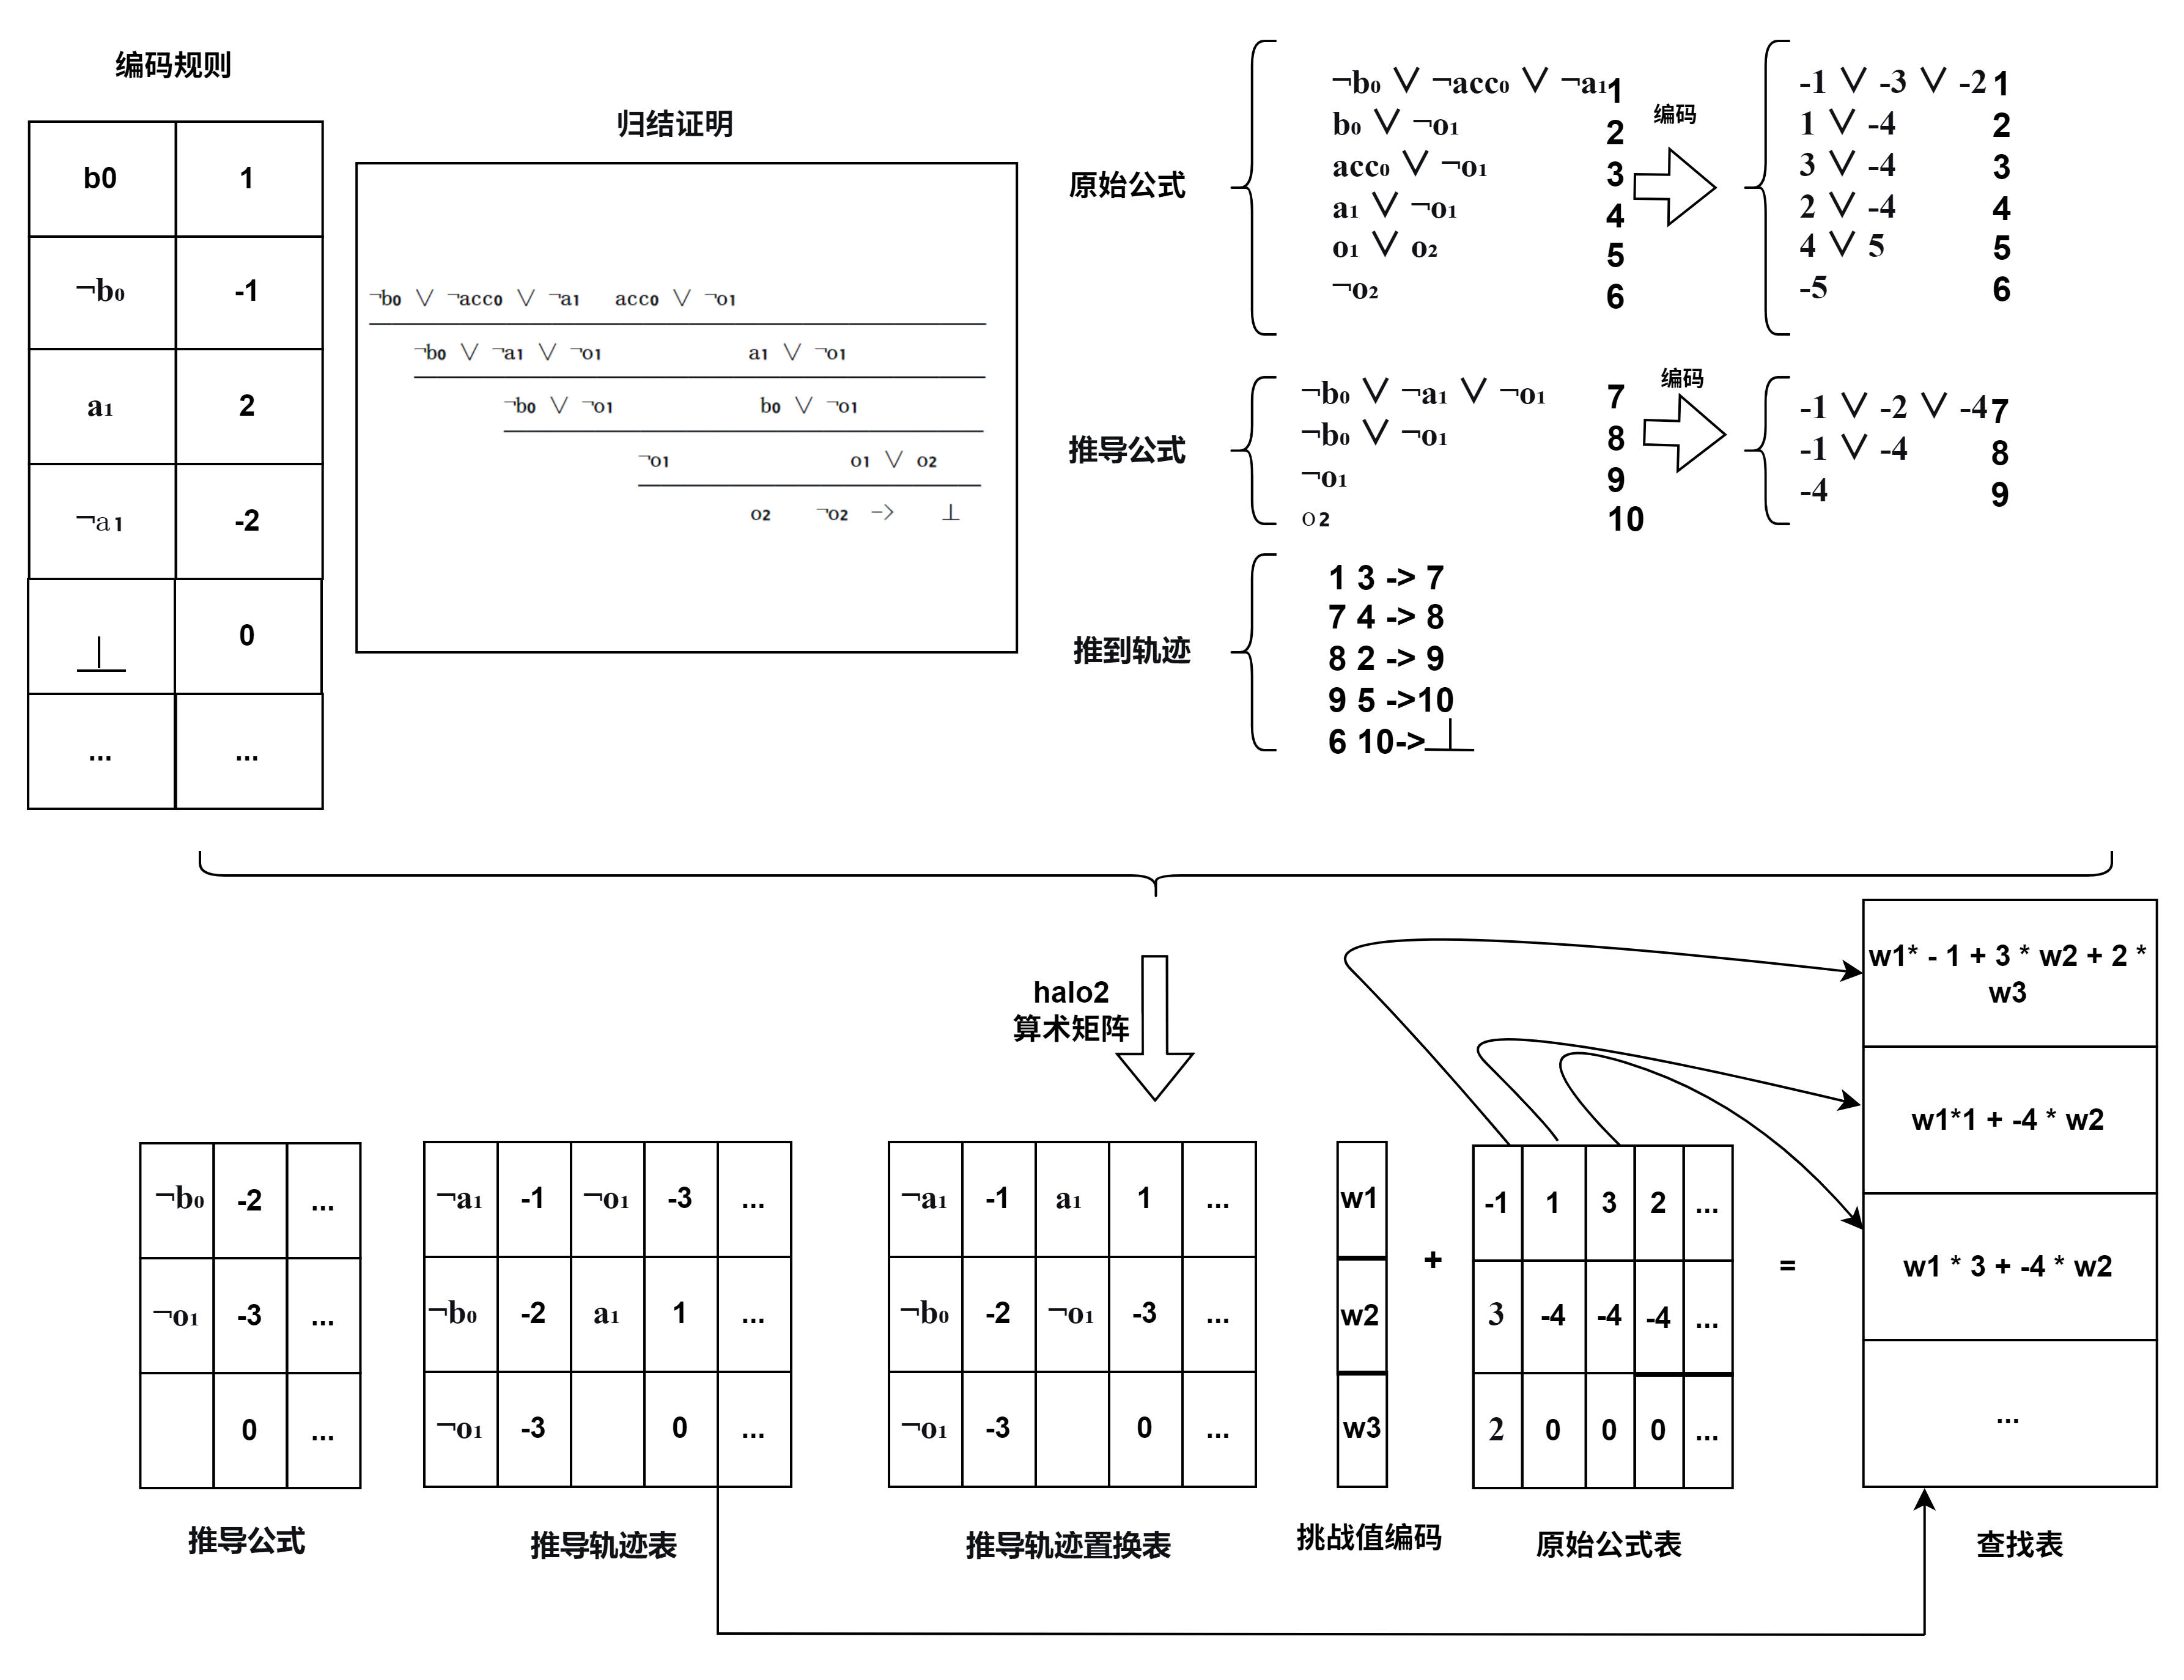
\includegraphics[width=0.95\linewidth]{figures/7.png}
    \bicaption{归结证明到halo2算术矩阵的构造流程}{Construction process from resolution proof to halo2 arithmetic matrix}
    \label{fig:unsat-matrix-construction}
\end{figure}

在矩阵构造阶段，编码后的归结证明被映射到halo2的表格结构中，如图下半部分所示。推导公式矩阵存储所有导出子句的内容，每行对应一个导出子句，列依次存储文字编码，长度不足最大宽度$W$的子句用零填充。推导轨迹表记录每个导出子句对应的两个父子句索引，用于验证归结步骤的正确性。推导轨迹置换表是轨迹表的重排列版本，其中每个父子句的枢轴变量被移动到固定的第二列位置，便于通过门约束$t'_{2i}[2] + t'_{2i-1}[2] = 0$直接验证枢轴变量的互补性。挑战值编码模块将变长子句压缩为单个有限域元素：验证者提供随机挑战值向量$\tilde{\chi} = (w_1, w_2, w_3, \ldots)$，每个子句通过线性组合$w_1 \cdot \ell_1 + w_2 \cdot \ell_2 + \ldots$编码为标量值，如图所示子句编码结果为$w_1 \cdot (-1) + 3 \cdot w_2 + 2 \cdot w_3$等形式。原始公式表以相同方式存储原始公式的所有子句。最右侧的查找表是约束系统的核心组件，通过将原始公式表和推导公式表的子句进行挑战值编码构成$L_1$，将轨迹表编码构成$L_2$，查找约束$L_2 \xrightarrow{\text{lookup}} L_1$确保轨迹中引用的每个子句都存在于已知子句集合中。整个矩阵构造的时间复杂度和空间复杂度均为$O((|F|+|D|+|T|) \cdot W)$，线性依赖于归结证明的规模，使得系统能够高效处理SAT实例。
\subsection{基于halo2的归结证明的约束建立}\label{sec:unsat-constraint-system}

在矩阵构造完成后，我们需要建立约束系统以强制执行第\ref{sec:sat-proof}节定义的归结证明验证关系。halo2提供三种约束机制：门约束（gate constraints）、复制约束（copy constraints）和查找约束（lookup constraints）。我们通过这些约束的组合，确保证明者提供的归结证明满足所有验证条件。

\textbf{轨迹包含性约束:}
第一个约束验证归结轨迹$T$中的每个子句都来自已知的子句集合$F \cup D$。由于采用了挑战值编码，这一验证简化为查找约束：
$$C_1: L_2 \xrightarrow{\text{lookup}} L_1$$
该约束要求$L_2$中的每个元素都存在于$L_1$中。在halo2后端，查找约束通过排列论证（permutation argument）实现，验证复杂度为$O(|L_2| \cdot \log |L_1|)$。$C_1$对应第\ref{sec:sat-proof}节验证关系(1)，确保归结过程仅使用有效子句。

\textbf{置乱一致性约束:}
置乱矩阵$T'$必须是轨迹$T$的重排列，即两者包含相同的子句集合，仅顺序可能不同。我们使用置乱约束：
$$C_2: T' \xrightarrow{\text{shuffle}} T$$
置乱约束在halo2中通过查找和置换的组合实现。该约束保证$T'$未引入额外子句或遗漏现有子句，确保后续约束基于完整且正确的轨迹集合。

\textbf{归结式正确性约束:}
归结规则要求导出子句$d_i$是父子句$t_{2i-1}$和$t_{2i}$在消去枢轴变量后的合并。在$T'$中，枢轴变量位于第二位置，因此我们验证$d_i$（移除索引$i^*$）等于$t'_{2i-1}$和$t'_{2i}$（移除索引$i^*$和第二位置元素）的并集：
$$C_3: (t'_{2i}, t'_{2i-1})_{-i^*, -\text{pos}_2} \xrightarrow{\text{lookup}} (D_i)_{-i^*}$$
这里$(...)_{-i^*, -\text{pos}_2}$表示移除索引和第二位置元素后的列向量。该约束对应验证关系(2)，确保归结式包含两个父子句的所有文字（除枢轴变量外）。

\textbf{枢轴变量互补性约束:}
归结要求父子句包含互补的枢轴变量。由于正文字编码为正数，负文字编码为负数，互补文字的和为零。我们定义门约束：
$$C_4: t'_{2i}[\text{pos}_2] + t'_{2i-1}[\text{pos}_2] = 0$$
其中$\text{pos}_2$表示第二位置（枢轴变量位置）。该约束确保$t'_{2i}$和$t'_{2i-1}$在该位置的值互为相反数，即一个为$\text{pivot}_i$，另一个为$\neg\text{pivot}_i$。

\textbf{轨迹长度约束:}
根据验证关系(3)，轨迹长度应为导出子句数量的两倍（每个导出需要两个父子句）。我们使用门约束：
$$C_5: 2 \cdot |D| = |T|$$
该约束通过instance列$I_{ns2}$（存储$|T|$）和公共参数$|D|$实现。

\textbf{空子句导出约束:}
归结证明的最终目标是导出空子句$\bot$。我们验证最后一个导出子句$d_{|D|}$为空：
$$C_6: D_{|D|} = 0_{\mathbb{F}}$$
通过查找fixed列$F_{ix}$实现。该约束对应验证关系(4)，确认不可满足性的证明完成。

约束系统$\{C_1, C_2, C_3, C_4, C_5, C_6\}$完整捕获了归结证明的语义。证明者必须同时满足所有约束才能通过验证，而每个约束都对应归结证明的一个必要条件，确保了验证的完备性和可靠性。

\subsection{性质证明}\label{sec:unsat-correctness}

本节从理论角度证明我们设计的halo2约束系统正确实现了UNSAT归结证明的零知识验证，同时满足完备性、可靠性和零知识性三个核心安全属性。

\begin{theorem}[UNSAT验证的完备性]
设$(F, D, T, T')$为不可满足公式$F$的有效归结证明。诚实的证明者能够构造满足约束$C_1$-$C_6$的halo2矩阵$M$，验证者以概率1接受该证明。
\end{theorem}

\begin{proof}
诚实证明者按照图\ref{fig:unsat-matrix-construction}构造矩阵$M$。由于归结证明$(F, D, T, T')$有效，满足第\ref{sec:sat-proof}节的所有验证关系。我们逐一验证每个约束：
\begin{itemize}
    \item $C_1$：由于$T \subseteq F \cup D$（验证关系(1)），$L_2$中每个元素（$T$的编码）必在$L_1$中（$F \cup D$的编码）。挑战值编码的唯一性保证相同子句编码相同。
    \item $C_2$：$T'$由$T$的子句重新排列构成（仅枢轴位置调整），两者包含相同子句集合。
    \item $C_3$：由验证关系(2)，$d_i$是$t_{2i-1}$和$t_{2i}$消去枢轴后的合并，因此$(t'_{2i}, t'_{2i-1})$移除枢轴后的并集等于$(D_i)$移除索引后的内容。
    \item $C_4$：由于$t_{2i-1}$和$t_{2i}$包含互补枢轴$\text{pivot}_i$和$\neg\text{pivot}_i$，编码为$+j$和$-j$，和为0。
    \item $C_5$：由验证关系(3)，$|T| = 2|D|$直接成立。
    \item $C_6$：由验证关系(4)，最后导出子句$d_{|D|} = \bot$，编码为$0_{\mathbb{F}}$。
\end{itemize}
因此，诚实证明者构造的矩阵满足所有约束，验证者接受。
\end{proof}

\begin{theorem}[UNSAT验证的可靠性]
若公式$F$可满足或证明$(F, D, T, T')$无效，恶意证明者构造满足约束$C_1$-$C_6$的矩阵$M$的概率至多为$\epsilon = W/|\mathbb{F}| + \text{negl}(|\mathbb{F}|)$，其中$W$为最大子句宽度，$\text{negl}$表示可忽略函数。
\end{theorem}

\begin{proof}
恶意证明者试图伪造证明有两种策略：
\begin{enumerate}
    \item \textbf{伪造归结步骤}：提供不满足归结规则的导出子句。约束$C_3$要求导出子句精确匹配父子句的归结式。若证明者提供错误的$d_i$，除非$\text{Encode}(d_i, \tilde{\chi}) = \text{Encode}(d'_i, \tilde{\chi})$（其中$d'_i$为正确归结式），否则$C_3$失败。根据Schwartz-Zippel引理，该概率至多$W/|\mathbb{F}|$。
    \item \textbf{伪造可满足公式的UNSAT证明}：若$F$可满足，不存在有效的归结到空子句的证明。证明者必须在某步违反归结规则或未导出空子句。约束$C_6$强制最后导出子句为空，而$C_1$-$C_4$确保所有导出步骤有效。若公式可满足，这些约束不可能同时成立，概率为0。
\end{enumerate}
综合两种情况，伪造成功概率至多为挑战值碰撞概率$W/|\mathbb{F}|$加上halo2底层的可靠性误差（通常为$\text{negl}(|\mathbb{F}|)$）。在标准参数下（$|\mathbb{F}| \approx 2^{256}$，$W < 10^3$），该概率可忽略。
\end{proof}

\begin{theorem}[UNSAT验证的零知识性]
我们的halo2协议是零知识的：验证者从协议交互中获得的信息，除了"$F$不可满足"这一事实外，不泄露关于$F$、$D$、$T$的任何额外信息。
\end{theorem}

\begin{proof}
零知识性通过模拟器论证证明。我们构造模拟器$\mathcal{S}$，仅知道"$F$不可满足"，能生成与真实协议交互在计算上不可区分的视图。

模拟器$\mathcal{S}$的构造：
\begin{enumerate}
    \item 随机选择有限域元素填充advice列（模拟$F, D, T, T'$）。
    \item 选择随机挑战值$\tilde{\chi}$（如真实协议）。
    \item 构造查找表$L_1, L_2$使得$C_1$成立（通过控制随机填充确保包含关系）。
    \item 调整advice列值使$C_2$-$C_6$成立（halo2的零知识模拟器能够在不知道witness的情况下生成满足约束的证明）。
\end{enumerate}

由于advice列对验证者不可见，验证者仅观察到：(1) instance列的公共参数$W, |T|$，(2) halo2证明的有效性。这些信息不依赖于$F$的具体结构，仅依赖于证明的存在性。根据halo2的零知识性质，模拟视图与真实视图在计算上不可区分，因此协议是零知识的。
\end{proof}

这三个定理共同确立了我们的UNSAT验证系统的安全性：诚实证明者总能成功证明，恶意证明者几乎不可能伪造，且验证过程不泄露任何私有信息。

\section{基于halo2的可满足性赋值的约束系统}

本节提出SAT可满足性赋值的零知识验证方案。我们设计双矩阵编码方案，通过互斥性约束确保变量赋值的唯一性和完整性，使得验证复杂度与公式规模线性相关。

\subsection{基于halo2的可满足性赋值的编码方案}\label{sec:sat-encoding-scheme}
可满足性验证的核心挑战在于确保变量赋值的唯一性和完整性。我们提出双矩阵编码方案，通过构造两个互斥矩阵分别存储赋值为0和1的变量。

\textbf{SAT验证的形式化定义:}
设布尔公式$F^*$为合取范式（CNF），由$n$个子句组成，即$F^* = \{f_1, f_2, \ldots, f_n\}$。布尔变量集合为$X = \{x_1, x_2, \ldots, x_m\}$。满足赋值$\alpha: X \rightarrow \{0, 1\}$是一个将每个变量映射到布尔值的函数，使得$F^*$中的每个子句至少有一个文字在$\alpha$下为真。

\textbf{文字到有限域的映射:}
与UNSAT验证类似，文字编码为有限域元素：正文字$x_j$编码为$\ell = j > 0$，负文字$\neg x_j$编码为$\ell = -j < 0$。赋值$\alpha(x_i) \in \{0, 1\}$直接作为有限域元素存储。

\textbf{双矩阵编码方案:}
双矩阵方案的关键洞察是：布尔赋值的唯一性等价于互斥性。我们构造两个矩阵$M_1$和$M_2$：
\begin{itemize}
    \item $M_1$：0-赋值矩阵，$M_1[j,k] = 1$当且仅当变量$x_i$的赋值为0
    \item $M_2$：1-赋值矩阵，$M_2[j,k] = 1$当且仅当变量$x_i$的赋值为1
\end{itemize}
其中$(j, k) = \text{position}(i) = (\lfloor i/L_m \rfloor, i \bmod L_m)$为变量$x_i$在矩阵中的位置。

通过单一的互斥性约束$M_1[j,k] + M_2[j,k] = 1$，可同时验证：
\begin{itemize}
    \item \textbf{唯一性}：变量不能同时被赋值为0和1
    \item \textbf{完整性}：每个变量必须被赋值
    \item \textbf{布尔性}：赋值只能是0或1
\end{itemize}

\textbf{子句满足性的编码:}
构造满足性矩阵$M_f$，维度为$|F^*| \times W$。对于子句$f_i$中位置$t$的文字$\ell$：
$$M_f[i,t] = \begin{cases}
\alpha(x_j) & \text{若$\ell = j > 0$（正文字）} \\
1 - \alpha(x_j) & \text{若$\ell = -j < 0$（负文字）}
\end{cases}$$
$M_f$的每行至少包含一个1当且仅当该子句被满足。

\textbf{编码效率:}
双矩阵方案将$m$个变量的验证简化为$O(m)$个统一形式的门约束，子句满足性验证复杂度为$O(|F^*| \cdot W)$。

\subsection{基于halo2的可满足性赋值的矩阵构造算法}\label{sec:sat-matrix-construction}

基于双矩阵编码方案，我们将SAT验证问题映射到halo2矩阵结构。矩阵构造的目标是将原始公式$F^*$和满足赋值$\alpha$转化为有限域上的表格表示，使得约束系统能够验证赋值的正确性。SAT验证的halo2矩阵$M \in \mathbb{F}^{n \times m}$包含以下组成部分：子句列为$|F^*|$个advice列，每列存储一个子句的文字编码；赋值矩阵$M_1$和$M_2$为两个advice矩阵，分别存储变量赋值为真和为假的标记；满足性矩阵$M_f$为instance矩阵，存储每个子句中各文字在当前赋值下的真值；查找表$L_1$仅包含元素1，用于验证子句满足性。

图\ref{fig:sat-matrix-construction}展示了从SAT公式和满足赋值到halo2算术矩阵的完整构造流程。在编码阶段，首先建立文字和真值到有限域元素的映射规则，如图左上角的编码表所示：正文字$b_0$编码为1，负文字$\neg b_0$编码为$-1$，正文字$a_1$编码为1，负文字$\neg a_1$编码为$-1$，布尔值$\text{true}$编码为1，$\text{false}$编码为0。图中央展示了一个具体的SAT验证实例：原始公式包含4个子句，分别为$b_0 \vee \neg o_1$、$acc_0 \vee \neg o_1$、$a_1 \vee \neg o_1$和$o_1 \vee o_2$，经编码后表示为$1 \vee -1$、$1 \vee -1$、$1 \vee -1$和$1 \vee 1$的形式；变量赋值为$b_0 = \text{true}$、$acc_0 = \text{true}$、$o_1 = \text{false}$、$o_2 = \text{true}$，在该赋值下每个子句中各文字的真值被计算并编码，例如第一个子句中$b_0$为真编码为1，$\neg o_1$为真编码为1，因此该行编码为$1 \vee 1$。

\begin{figure}[htbp]
    \centering
    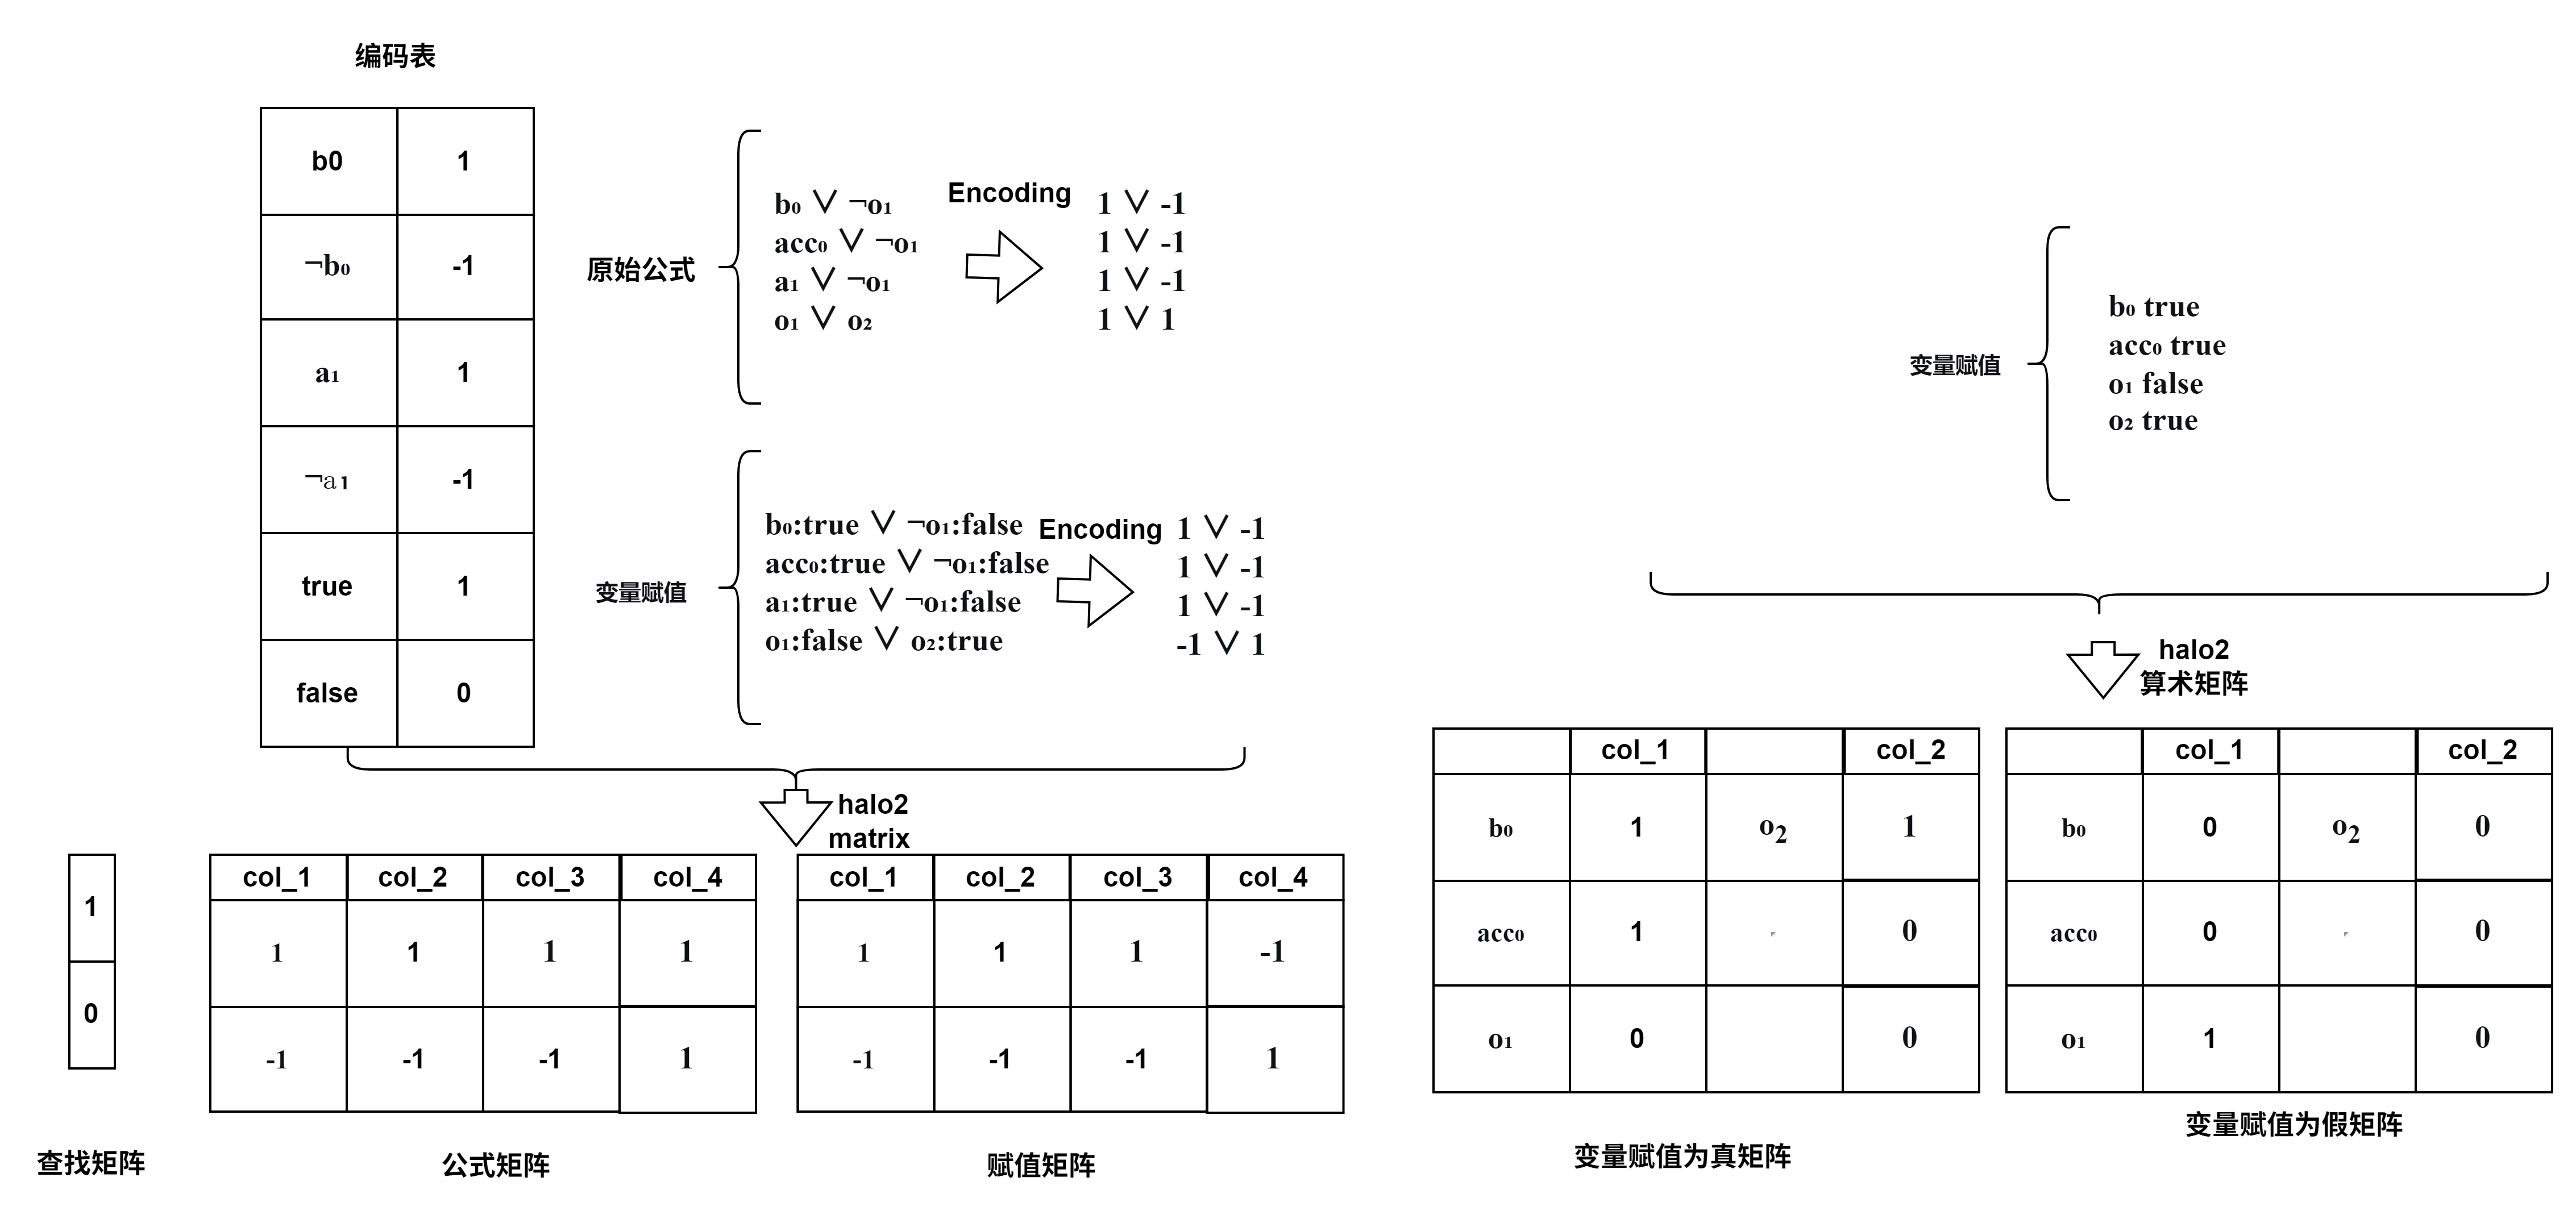
\includegraphics[width=0.95\linewidth]{figures/8.png}
    \bicaption{SAT公式到halo2算术矩阵的构造流程}{Construction process from SAT formula to halo2 arithmetic matrix}
    \label{fig:sat-matrix-construction}
\end{figure}

在矩阵构造阶段，编码后的公式和赋值被映射到halo2的表格结构中，如图下半部分所示。查找矩阵位于最左侧，仅包含元素1和0两行，用于后续的查找约束验证。公式矩阵存储原始公式中每个子句的文字编码，每行对应一个子句，列col\_1至col\_4依次存储子句中的文字，图中示例显示第一行为$(1, 1, 1, 1)$，第二行为$(-1, -1, -1, 1)$，表示各子句的文字编码值。赋值矩阵$M_f$存储每个子句中各文字在当前赋值下的真值，其结构

\subsection{基于halo2的可满足性赋值的约束建立}\label{sec:sat-constraint-verification}

在矩阵构造完成后，我们建立约束系统验证第\ref{sec:sat-proof}节定义的SAT验证关系。与UNSAT验证相比，SAT验证的约束系统更为简洁，主要包含赋值唯一性约束和子句满足性约束两类。

\textbf{赋值唯一性约束:}
双矩阵方案的核心约束是互斥性约束。对于赋值矩阵$M_1$和$M_2$的每个对应位置$(j,k)$，我们要求：
$$C_1: M_1[j,k] + M_2[j,k] = 1, \quad \forall j \in [1, L_m], \forall k \in [1, n_{\text{cols}}]$$
这是一个门约束，在halo2中通过算术门实现。该约束同时确保三个性质：
\begin{itemize}
    \item \textbf{布尔性}：由于$M_1, M_2$的值域为$\{0,1\}$（由构造保证），$M_1 + M_2 = 1$隐含$M_1, M_2 \in \{0,1\}$。
    \item \textbf{互斥性}：$M_1[j,k]$和$M_2[j,k]$不能同时为1，确保变量不会同时被赋值为0和1。
    \item \textbf{完整性}：$M_1[j,k]$和$M_2[j,k]$不能同时为0，确保每个变量必被赋值。
\end{itemize}
约束$C_1$对应第\ref{sec:sat-proof}节验证关系(1)，确保赋值$\alpha$为每个变量提供唯一的布尔值。约束数量为$O(L_m \cdot n_{\text{cols}}) = O(m)$，与变量数量线性相关，但由于约束形式统一，验证效率高。

\textbf{子句满足性约束:}
满足性矩阵$M_f$的每行对应公式$F^*$的一个子句。根据验证关系(2)，每个子句必须至少有一个文字在赋值下为真，即$M_f$的每行至少包含一个1。我们使用查找约束：
$$C_2: M_f \xrightarrow{\text{lookup}} L_1$$
该约束要求$M_f$中的每个元素都存在于查找表$L_1 = \{1\}$中。由于查找约束是逐元素验证的，$M_f[i,t] \in L_1$意味着$M_f[i,t] = 1$。因此，若$M_f$的某行全为0（子句未被满足），该行的查找会失败，约束不成立。

查找约束的巧妙之处在于：它不仅验证每行至少有一个1（子句满足性），还隐式验证$M_f$的所有元素都为0或1（布尔性）。这种双重验证避免了额外的布尔约束，提升了系统效率。

\textbf{约束系统的完备性分析:}
约束$\{C_1, C_2\}$完整捕获了SAT验证的所有必要条件：
\begin{itemize}
    \item $C_1$确保赋值$\alpha$的唯一性、完整性和布尔性（验证关系(1)）。
    \item $C_2$确保每个子句在赋值下至少有一个文字为真（验证关系(2)）。
\end{itemize}
若证明者提供的赋值不满足公式，必在某个子句处违反$C_2$；若赋值不唯一或不完整，必违反$C_1$。因此，满足$C_1$和$C_2$的赋值必是有效的满足赋值。

\textbf{约束验证的计算复杂度:}
门约束$C_1$的验证涉及$O(m)$个位置，每个位置的验证为常数时间，总复杂度$O(m)$。查找约束$C_2$涉及$M_f$的$O(|F^*| \cdot W)$个元素，查找到$L_1$（仅一个元素）的复杂度为$O(|F^*| \cdot W)$。综合而言，约束验证的总复杂度为$O(m + |F^*| \cdot W)$，与公式和赋值的规模线性相关，远优于指数级的穷举验证。

\subsection{性质证明}\label{sec:sat-security}

本节从理论角度证明SAT验证系统的安全性，包括完备性、可靠性和零知识性。与UNSAT验证类似，我们通过形式化定理和严格证明确立系统的安全属性。

\begin{theorem}[SAT验证的完备性]
设$\alpha$为可满足公式$F^*$的有效满足赋值。诚实的证明者能够构造满足约束$C_1$-$C_2$的halo2矩阵$M$，验证者以概率1接受该赋值。
\end{theorem}

\begin{proof}
诚实证明者按照图\ref{fig:sat-matrix-construction}构造矩阵$M$。由于$\alpha$为有效满足赋值，满足第\ref{sec:sat-proof}节的验证关系(1)和(2)。我们验证每个约束：
\begin{itemize}
    \item $C_1$：对于每个变量$x_i$，位置$(j,k) = \text{position}(i)$处，$M_1[j,k] = 1 - \alpha(x_i)$，$M_2[j,k] = \alpha(x_i)$。因此$M_1[j,k] + M_2[j,k] = (1 - \alpha(x_i)) + \alpha(x_i) = 1$。约束成立。
    \item $C_2$：由验证关系(2)，每个子句$f_i \in F^*$至少有一个文字$\ell$在赋值下为真。根据$M_f$的构造规则，该文字对应的位置$(i,t)$满足$M_f[i,t] = 1$。因此$M_f$的第$i$行至少包含一个1，该行的查找到$L_1 = \{1\}$成功。约束成立。
\end{itemize}
因此，诚实证明者构造的矩阵满足所有约束，验证者接受。
\end{proof}

\begin{theorem}[SAT验证的可靠性]
若公式$F^*$不可满足或赋值$\alpha$无效，恶意证明者构造满足约束$C_1$-$C_2$的矩阵$M$的概率至多为$\text{negl}(|\mathbb{F}|)$（可忽略函数）。
\end{theorem}

\begin{proof}
恶意证明者试图伪造有效赋值有两种策略：
\begin{enumerate}
    \item \textbf{伪造不可满足公式的SAT赋值}：若$F^*$不可满足，任何赋值$\alpha$都无法使所有子句同时为真。存在子句$f_i$在$\alpha$下全部文字为假，对应$M_f$的第$i$行全为0。该行查找$L_1 = \{1\}$失败，$C_2$不成立。证明者无法通过验证。
    \item \textbf{提供不唯一或不完整的赋值}：若赋值未定义某变量$x_i$或为其提供多个值，对应位置$(j,k)$的$M_1[j,k] + M_2[j,k] \neq 1$。具体而言：
    \begin{itemize}
        \item 若$x_i$未赋值（$M_1[j,k] = M_2[j,k] = 0$）：$M_1[j,k] + M_2[j,k] = 0 \neq 1$，$C_1$失败。
        \item 若$x_i$被赋值为0和1（$M_1[j,k] = M_2[j,k] = 1$）：$M_1[j,k] + M_2[j,k] = 2 \neq 1$，$C_1$失败。
    \end{itemize}
    证明者无法通过验证。
\end{enumerate}
唯一的攻击向量是利用halo2底层的可靠性漏洞（如伪造证明），但根据halo2的安全性质，该概率为$\text{negl}(|\mathbb{F}|)$，在实际参数下可忽略。因此，伪造成功概率可忽略。
\end{proof}

\begin{theorem}[SAT验证的零知识性]
我们的halo2协议是零知识的：验证者从协议交互中获得的信息，除了"$F^*$可满足"这一事实外，不泄露关于$F^*$或赋值$\alpha$的任何额外信息。
\end{theorem}

\begin{proof}
零知识性通过模拟器论证证明。我们构造模拟器$\mathcal{S}$，仅知道"$F^*$可满足"及公共参数（$m, |F^*|, W$），能生成与真实协议交互在计算上不可区分的视图。

模拟器$\mathcal{S}$的构造：
\begin{enumerate}
    \item \textbf{模拟赋值矩阵}：随机生成$M_1, M_2$，满足$M_1[j,k] + M_2[j,k] = 1$（通过随机选择$M_1[j,k] \in \{0,1\}$，设$M_2[j,k] = 1 - M_1[j,k]$）。这些矩阵在advice列中，验证者不可见。
    \item \textbf{模拟满足性矩阵}：随机生成$M_f$，确保每行至少有一个1（通过在每行随机位置填充1）。$M_f$在instance列中，验证者可见，但由于其构造随机，不泄露具体赋值信息。
    \item \textbf{模拟约束满足}：利用halo2的零知识模拟器，生成满足$C_1$-$C_2$的证明，而无需知道真实的$\alpha$。
\end{enumerate}

验证者观察到的信息包括：
\begin{itemize}
    \item \textbf{Instance列}：$M_f$的值（满足模式）和公共参数$L_m$。$M_f$的随机构造确保其分布与真实满足性矩阵在计算上不可区分。
    \item \textbf{halo2证明}：证明的有效性（通过零知识模拟器生成）。
\end{itemize}

关键观察：$M_f$仅揭示"每个子句被满足"这一事实，而不揭示哪个文字使子句为真。由于子句可能有多个文字为真，$M_f$中1的位置分布依赖于具体赋值，但模拟器通过随机选择1的位置，生成与真实分布无法区分的$M_f$。

根据halo2的零知识性质和模拟器的构造，模拟视图与真实视图在计算上不可区分。因此，协议是零知识的，验证者无法从交互中提取关于$F^*$或$\alpha$的额外信息。
\end{proof}

这三个定理共同确立了SAT验证系统的安全性：诚实证明者总能成功证明有效赋值，恶意证明者几乎不可能伪造无效赋值或不可满足公式的证明，且验证过程保持完全的零知识性，不泄露任何私有信息。
